\subsection{Synthetische Daten}\label{sec:synthetic_data}

Bei einem synthetischen Datenbestand handelt es sich um einen künstlich erzeugten Datenbestand, welcher die gleichen statistischen Merkmale wie der ursprüngliche Datenbestand enthält.
Statistische Abfragen oder auch komplexere Modelle, wie neuronale Netze, sollen demnach bei beiden Datenbeständen vergleichbare Ergebnisse liefern.

Bisher wurde Differential Privacy für einzelne Abfragen genutzt.
Es gibt jedoch auch Verfahren, welche es ermöglichen, eine synthetische Menge an Datensätzen zu veröffentlichen, welcher mit Differential Privacy geschützt werden.
Hardt \etal \cite{P-90} stellen solch ein Verfahren vor, welches MWEM genannt wird.
Dieses basiert auf Marginalverteilungen, auch Randverteilungen genannt, von verschiedenen Attributen zueinander.
Dabei handelt es sich um Anzahlen verschiedener Attributwerte eines Attributs in Kombination mit den Anzahlen verschiedener Attributwerte eines anderen Attributes.
Einzelne Werte der Marginalverteilungen werden auch Marginalhäufigkeiten genannt.
Tabelle \ref{tab:marginals} zeigt, wie ein Beispiel von Marginalverteilungen zwischen den Attributen \dq A\dq\ und \dq B\dq, welche jeweils zwei unterschiedliche Attributwerte annehmen können.
Stetige Werte müssten vorher in verschiedene Klassen gruppiert werden.

% Please add the following required packages to your document preamble:
% \usepackage[table,xcdraw]{xcolor}
% If you use beamer only pass "xcolor=table" option, i.e. \documentclass[xcolor=table]{beamer}
\begin{table}[!htb]
\centering
\begin{tabular}{|
>{\columncolor[HTML]{CBCEFB}}l |l|l|l|}
\hline
                   & \cellcolor[HTML]{CBCEFB}Attributwert \dq $A_{1}$\dq & \cellcolor[HTML]{CBCEFB}Attributwert \dq $A_{2}$\dq & \cellcolor[HTML]{CBCEFB}Marginalverteilung \\ \hline
Attributwert \dq $B_{1}$\dq    & 10                                      & 5                                       & 15                                         \\ \hline
Attributwert \dq $B_{2}$\dq    & 13                                      & 4                                       & 17                                         \\ \hline
Marginalverteilung & 23                                      & 9                                       & 32                                         \\ \hline
\end{tabular}
\caption{Beispiel Marginalverteilungen\cite{D-titanic}}
\label{tab:marginals}
\end{table}

Um eine Datenmenge umzuwandeln, wird eine Datenmenge $D'$ mit der gleichen Anzahl an Elementen wie die ursprüngliche Datenmenge $D$ initialisiert, wobei die Initialwerte der Attribute mittels einer Gleichverteilung über alle potenziellen Attributwerte des jeweiligen Attributes ermittelt werden.
Das Verfahren besteht aus 3 Schritten, welche iterativ wiederholt werden können, um die künstliche Datenmenge $D'$ an die echte Datenmenge $D$ anzugleichen:
\begin{compactenum}
    \item \textbf{Wahl einer Anfrage:} Aus allen Marginalhäufigkeiten der ursprünglichen Datenmenge, wird mittels Exponential-Mechanismus die Marginalhäufigkeit gewählt, die den größten Unterschied zwischen den Eingaben $D'$ und $D$ besitzt.
    Die Bewertungsfunktion $u$ des Exponential-Mechanismus bewertet folglich die Differenzen der Marginalverteilungen der beiden Datenmengen (originale Datenmenge und synthetische Datenmenge).
    \item \textbf{Verrauschen:} Mittels Laplace-Mechanismus wird nun das Ergebnis der gewählten Marginalverteilung aus Schritt 1 verrauscht.
    \item \textbf{Anpassen von $D'$:} Abhängig von dem verrauschten Ergebnis der gewählten Marginalverteilung, werden die Attributwerte von $D'$ so angepasst, dass die Marginalverteilungen sich angleichen.
\end{compactenum}
Nach Beendigung des Algorithmus, ist $D'$ eine synthetische Datenmenge, welche die originale Datenmenge $D$ mit Differential Privacy abbildet.

Die Erzeugung synthetischer Daten wurde im Jahre 2016 maßgeblich durch die Generative Adversarial Network Architektur, auch GAN genannt, beeinflusst \cite{P-86}. 
Bei dieser Architektur gibt es zwei gegensätzliche neuronale Netzwerke, der Generator und der Diskriminator. 
Der Diskriminator lernt dabei, zwischen echten Daten und nicht echten Daten zu unterscheiden, welche abwechselnd von dem echten Datenbestand und von dem Generator kommen.
Im Gegensatz dazu, versucht der Generator, Datensätze zu erzeugen, die den Diskriminator täuschen. 
Der Diskriminator kann dabei zwei Verlustfunktionen haben, einmal für sich selber und einmal für den Generator.
Die Verlustfunktion des Generators kann dabei durch den Generator backpropagiert werden, wodurch dieser immer realistischere Datensätze generiert.
Im besten Falle, erzeugt der Generator nach dem Training Datensätze, die so echt wirken, dass der Diskriminator diese nicht mehr unterscheiden kann.
Folglich erzeugt der Generator synthetische Daten, welche die statistischen Strukturen der originalen Daten enthalten.
Abbildung \ref{fig:gan} zeigt die bereits beschriebene Architektur.

\begin{figure}[!htb]
    \centering
    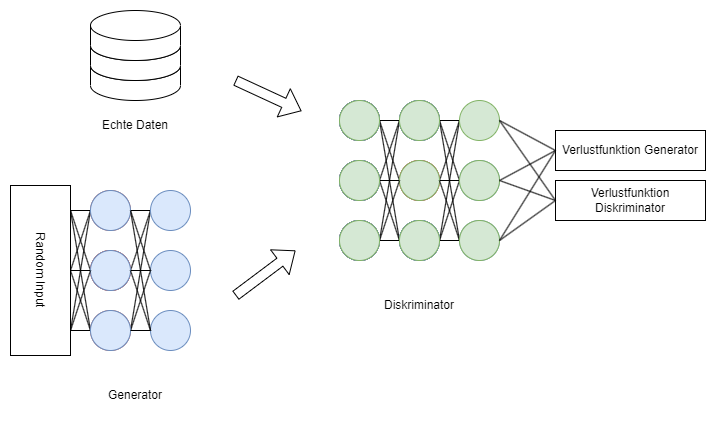
\includegraphics[width=14cm]{figures/gan}
    \caption{Generative Adversarial Network nach \cite{P-86}}
    \label{fig:gan}
\end{figure} 

Die Erzeugung von Daten mittels GANs kann nicht nur für Angriffe genutzt werden (siehe Kapitel \ref{sec:angriffe}), sondern auch für das Training von neuronalen Netzen.
Eine Erweiterung der GANs ist das sogenannte Wasserstein GAN oder auch kurz WGAN \cite{P-92}. 
Standardmäßig kann bei GANs der Fall auftreten, dass die erzeugten Daten nicht jeden Teil einer Verteilung abbilden, sondern nur einen Teil, \zB den am häufigsten vorkommenden Datensatz.
Um dieses Problem zu mindern, wird beim WGAN die Verlustfunktion des Diskriminators verändert. 
Anstatt einer binären Klassifikation (echt oder unecht), wird die Wasserstein-Distanz genutzt, welche angibt, wie viel Arbeit benötigt wird, um eine Verteilung in eine andere Verteilung zu transformieren. 
Die Wasserstein-Distanz gleicht der Earth-Mover-Distanz aus Kapitel \ref{sec:anonymisierung}.
Diese Metrik als Verlustfunktion ist jedoch nur nützlich, wenn nicht mit einzelnen Datensätzen, sondern jeweils mit Batches trainiert wird.
Der Austausch der Verlustfunktion sorgt dafür, dass der Generator Daten aus der ganzen Verteilung der Daten nachstellen muss und nicht nur aus einem Teil dieser.


Xie \etal \cite{P-70} stellen eine besondere Form des GANs vor, das sogenannte Differentially Private Generative Adversarial Network oder kurz DPGAN.
Dieses DPGAN nutzt als Basis das WGAN, fügt jedoch bei Berechnung der Verlustfunktion (Wasserstein-Distanz) Rauschen mittels des Gauß-Mechanismus aus Kapitel \ref{sec:dp} hinzu.
Durch die Eigenschaft, dass Differential Privacy resistent gegenüber Nachbearbeitung ist, kann auch garantiert werden, dass die Gradienten, die im Generator ankommen, mittels Differential Privacy geschützt sind.
Die Autoren können zeigen, dass es möglich ist, Bilder der MNIST Datenmenge \cite{D-MNIST} zu erzeugen.
Abbildung \ref{fig:dpgan} zeigt diese Erzeugung mit unterschiedlichen $\epsilon$ Werten.
Es ist zu sehen, dass bei kleiner werdendem $\epsilon$, die Qualität der Bilder schlechter wird und auch mehr Daten der falschen Klasse erzeugt werden. 
Bei $\epsilon=9,6$ ist die Anzahl an Daten mit falschem Label größer, als die Anzahl der Daten mit richtigem Label.
Folglich ist die Wahl von $\epsilon$ entscheidend, wie gut die synthetischen Daten die Originaldaten wiedergeben.
Die Wahl muss von $\epsilon$ muss dabei für jeden Use Case neu evaluiert werden.

\begin{figure}[!htb]
    \centering
    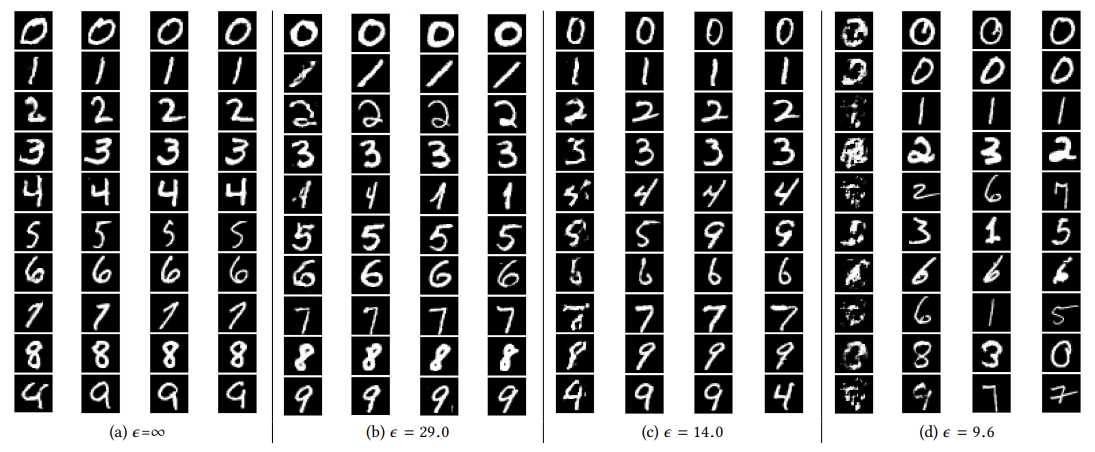
\includegraphics[width=\textwidth]{figures/dpgan}
    \caption{Synthetische MNIST Datenmenge mittels DPGAN \cite{P-70}}
    \label{fig:dpgan}
\end{figure} 

Jordon \etal \cite{P-68} stellten eine alternative Form des GANs vor, welches ebenfalls synthetische Daten erzeugt. 
Dieses nutzt das Private Aggregation of Teacher Ensembles Framework, kurz PATE, welches in Kapitel \ref{sec:pate} im Detail beleuchtet wird.
Bei der PATE-Architektur wird der Datenbestand in verschiedene Teildatenmengen unterteilt. 
Verschiedene Modelle, die sogenannten Lehrer oder Teacher Modelle, lernen die Klassifikation jeweils an einer der unterschiedlichen Teildatenmengen.
Ein weiteres Modell, welches Schüler oder Student Modell genannt wird, kann nun mittels des Exponential-Mechanismus aus \ref{sec:dp} aus den aggregierten Vorhersagen der Lehrer Modelle, eine Klasse vorhersagen.
Das PATE-GAN nutzt die PATE-Architektur für den Diskriminator, welcher ein binärer Klassifikator ist.
Wie das DPGAN, nutzt auch das PATE-GAN die Resistenz gegenüber Nachbearbeitungen von Differential Privacy aus, um Differential Privacy auch für die synthetischen Daten zu garantieren.


Ein weiterer Algorithmus, welcher kein GAN zur Erzeugung künstlicher Daten nutzt, ist NIST-MST von McKenna \etal \cite{P-95}.
Mit NIST-MST gewannen McKenna \etal die \textit{Differential Privacy Synthetic Data Competition}, welche vom National Institute of Standards and Technology der USA ausgetragen wurde.
Neben NIST-MST, welcher auf den obigen Wettbewerb angepasst wurde, gibt es noch MST für generelle Anwendungsfälle.
Die MST Methode basiert, wie MWEM \cite{P-90}, auf Marginalverteilungen.
MST besteht dabei aus 3 Schritten \cite{P-95}:
\begin{compactenum}
    \item \textbf{Wahl von Marginalverteilungen:} Aus dem Datenbestand, über den synthetische Daten erzeugt werden, können mehrere Marginalverteilungen gewählt werden. Dabei sollten die wichtigsten Zusammenhänge und Abhängigkeiten des Datenbestands in diesen vorkommen. Es wird deshalb empfohlen, dass ein Fachexperte die Marginalverteilungen aussucht.
    \item \textbf{Zählen der Marginalverteilungen:} Marginalverteilungen enthalten die Anzahl von Attributwerten eines Attributes in Abhängigkeit von den Attributwerten eines anderen Attributes. Um die Vertraulichkeit der Daten mittels Differential Privacy zu schützen, werden die unterschiedlichen Anzahlen der Variablen mittels Gauß-Mechanismus verrauscht.
    \item \textbf{Erzeugung der Daten:} MST nutzt ein Tool namens Private-PGM \cite{P-97}, welches von den gleichen Autoren stammt, um einen künstlichen Datenbestand zu erzeugen. Dabei sollen die Marginalverteilungen des künstlichen Datenbestands möglichst nahe an den gemessenen Marginalverteilungen liegen.
\end{compactenum}
Die MST Methode ähnelt der MWEM Methode, jedoch gibt es einige Unterschiede.
MWEM ist ein iterativer Algorithmus, welcher in jeder Iteration die Marginalhäufigkeit mit der größten Differenz zwischen originalem Datenbestand $D$ und synthetischem Datenbestand $D'$ wählt und die Attributwerte des synthetischen Datenbestands so anpasst, dass diese sich der Marginalhäufigkeit des originalen Datensatzes angleicht.
MST hingegen stellt mit dem Tool Private-PGM \cite{P-97} ein Optimierungsproblem auf, welches versucht, einen Datenbestand zu finden, dessen Marginalverteilungen möglichst Nahe an den gemessenen Marginalverteilungen des originalen Datenbestands liegt.